% !TEX TS-program = XeLaTeX
% use the following command:
% all document files must be coded in UTF-8
\documentclass[portuguese]{textolivre}
% build HTML with: make4ht -e build.lua -c textolivre.cfg -x -u article "fn-in,svg,pic-align"

\journalname{Texto Livre}
\thevolume{19}
%\thenumber{1} % old template
\theyear{2026}
\receiveddate{\DTMdisplaydate{2026}{3}{16}{-1}} % YYYY MM DD
\accepteddate{\DTMdisplaydate{2026}{4}{22}{-1}}
\publisheddate{\DTMdisplaydate{2026}{10}{21}{-1}}
\corrauthor{Letícia Moraes}
\articledoi{10.1590/1983-3652.2026.64149}
%\articleid{NNNN} % if the article ID is not the last 5 numbers of its DOI, provide it using \articleid{} commmand 
% list of available sesscions in the journal: articles, dossier, reports, essays, reviews, interviews, editorial
\articlesessionname{articles}
\runningauthor{Moraes} 
%\editorname{Leonardo Araújo} % old template
\sectioneditorname{Daniervelin Pereira~\orcid{0000-0003-1861-3609}}
\layouteditorname{Rayany Chaves~\orcid{0009-0007-0028-484X}}

\title{Inteligência artificial, epistemologia e raça: questões semióticas}
\othertitle{Artificial Intelligence, Epistemology, and Race: Semiotic Issues}
% if there is a third language title, add here:
%\othertitle{Artikelvorlage zur Einreichung beim Texto Livre Journal}

\author[1]{Letícia Moraes~\orcid{0000-0002-4642-5974}\thanks{Email: \href{mailto:lesemiotica@gmail.com}{lesemiotica@gmail.com}}}
\affil[1]{Universidade Federal da Paraíba, Centro de Ciências Humanas, Letras e Artes, Departamento de Linguística e Língua Portuguesa, João Pessoa, Paraíba, Brasil.}

\addbibresource{article.bib}
% use biber instead of bibtex
% $ biber article

% used to create dummy text for the template file
\definecolor{dark-gray}{gray}{0.35} % color used to display dummy texts
\usepackage{lipsum}
\SetLipsumParListSurrounders{\colorlet{oldcolor}{.}\color{dark-gray}}{\color{oldcolor}}

% used here only to provide the XeLaTeX and BibTeX logos
\usepackage{hologo}

% if you use multirows in a table, include the multirow package
\usepackage{multirow}

% provides sidewaysfigure environment
\usepackage{rotating}

% CUSTOM EPIGRAPH - BEGIN 
%%% https://tex.stackexchange.com/questions/193178/specific-epigraph-style
\usepackage{epigraph}
\renewcommand\textflush{flushright}
\makeatletter
\newlength\epitextskip
\pretocmd{\@epitext}{\em}{}{}
\apptocmd{\@epitext}{\em}{}{}
\patchcmd{\epigraph}{\@epitext{#1}\\}{\@epitext{#1}\\[\epitextskip]}{}{}
\makeatother
\setlength\epigraphrule{0pt}
\setlength\epitextskip{0.5ex}
\setlength\epigraphwidth{.7\textwidth}
% CUSTOM EPIGRAPH - END

% to use IPA symbols in unicode add
%\usepackage{fontspec}
%\newfontfamily\ipafont{CMU Serif}
%\newcommand{\ipa}[1]{{\ipafont #1}}
% and in the text you may use the \ipa{...} command passing the symbols in unicode

% LANGUAGE - BEGIN
% ARABIC
% for languages that use special fonts, you must provide the typeface that will be used
% \setotherlanguage{arabic}
% \newfontfamily\arabicfont[Script=Arabic]{Amiri}
% \newfontfamily\arabicfontsf[Script=Arabic]{Amiri}
% \newfontfamily\arabicfonttt[Script=Arabic]{Amiri}
%
% in the article, to add arabic text use: \textlang{arabic}{ ... }
%
% RUSSIAN
% for russian text we also need to define fonts with support for Cyrillic script
% \usepackage{fontspec}
% \setotherlanguage{russian}
% \newfontfamily\cyrillicfont{Times New Roman}
% \newfontfamily\cyrillicfontsf{Times New Roman}[Script=Cyrillic]
% \newfontfamily\cyrillicfonttt{Times New Roman}[Script=Cyrillic]
%
% in the text use \begin{russian} ... \end{russian}
% LANGUAGE - END

% EMOJIS - BEGIN
% to use emoticons in your manuscript
% https://stackoverflow.com/questions/190145/how-to-insert-emoticons-in-latex/57076064
% using font Symbola, which has full support
% the font may be downloaded at:
% https://dn-works.com/ufas/
% add to preamble:
% \newfontfamily\Symbola{Symbola}
% in the text use:
% {\Symbola }
% EMOJIS - END

% LABEL REFERENCE TO DESCRIPTIVE LIST - BEGIN
% reference itens in a descriptive list using their labels instead of numbers
% insert the code below in the preambule:
%\makeatletter
%\let\orgdescriptionlabel\descriptionlabel
%\renewcommand*{\descriptionlabel}[1]{%
%  \let\orglabel\label
%  \let\label\@gobble
%  \phantomsection
%  \edef\@currentlabel{#1\unskip}%
%  \let\label\orglabel
%  \orgdescriptionlabel{#1}%
%}
%\makeatother
%
% in your document, use as illustraded here:
%\begin{description}
%  \item[first\label{itm1}] this is only an example;
%  % ...  add more items
%\end{description}
% LABEL REFERENCE TO DESCRIPTIVE LIST - END


% add line numbers for submission
%\usepackage{lineno}
%\linenumbers

\begin{document}
\maketitle

\begin{polyabstract}
\begin{abstract}
Parte-se do discurso de ruptura frequentemente associado à inteligência artificial, argumentando-se que modelos de geração de imagens tendem a reutilizar formas e sentidos anteriores à própria existência dessas tecnologias. Analisam-se os mecanismos pelos quais o viés racial se manifesta nas imagens produzidas pelo DALL·E. Para isso, foram realizados testes que articulam a figurativização de corpos humanos em profissões socialmente investidas de maior ou menor prestígio — como médico(a), professor(a) universitário(a), engenheiro(a) civil, faxineiro(a) de hospital, pedreiro(a) e catador(a) de lixo —, observando-se as regularidades emergentes na distribuição figurativa. Os resultados indicam que, por meio de operações estatísticas sobre big data, o sistema organiza e hierarquiza combinações recorrentes de figuras e traços visuais, associando profissões socialmente desvalorizadas com corpos negros e determinadas marcas plásticas, como cabelos crespos escondidos. Tais marcas tendem a estar ausentes nas representações associadas a profissões de maior prestígio. Observa-se também uma distinção aspectual relevante: enquanto os corpos negros vinculados às profissões desvalorizadas são figurativizados sob a modalidade do fazer, em plena atividade laboral, os corpos associados às ocupações prestigiadas são modalizados predominantemente pelo ser, em posições corporais estáticas. Essa configuração dialoga com padrões historicamente sedimentados na iconografia ocidental, contribuindo para a estabilização de uma norma semiótica racista. O artigo defende, portanto, a necessidade de uma semiótica da inteligência artificial, capaz de analisar criticamente as significações geradas nesses sistemas e de contribuir para o desenvolvimento de tecnologias mais plurais a partir das epistemologias do Sul.

\keywords{Semiótica discursiva \sep Inteligência artificial generativa \sep Viés racial \sep Big data \sep Epistemologias do Sul}
\end{abstract}

\begin{english}
\begin{abstract}
This article challenges the discourse of rupture often associated with artificial intelligence, arguing that image generation models tend to recycle forms and meanings that predate the technologies themselves. It examines the mechanisms through which racial bias manifests in images produced by DALL·E. To this end, a series of tests were conducted linking the figurativization of human bodies to professions socially invested with varying degrees of prestige—such as doctor, university professor, civil engineer, hospital cleaner, construction worker, and waste picker—observing the regularities that emerged in the figurative distribution. The results indicate that, through statistical operations, the system organizes and hierarchizes recurrent combinations of figures and visual traits, associating socially devalued professions with Black bodies and specific plastic markers, such as concealed curly hair. Such markers tend to be absent from representations associated with higher-prestige professions. A relevant aspectual distinction is also observed: while Black bodies linked to devalued professions are figurativized under the modality of doing, amid labor activity, bodies associated with prestigious occupations are predominantly modalized through being, in static bodily positions. This configuration resonates with historically sedimented patterns in Western iconography, contributing to the stabilization of a racist semiotic norm. The article therefore argues for the need to develop a semiotics of artificial intelligence capable of critically analyzing the meanings generated by these systems and contributing to the development of more plural technologies grounded in epistemological perspectives from the Global South.

\keywords{Discursive semiotics \sep Generative AI \sep Racial bias \sep Big data \sep Epistemologies of the South}
\end{abstract}
\end{english}
% if there is another abstract, insert it here using the same scheme
\end{polyabstract}

\section{Prólogo}\label{sec-intro}

As primeiras décadas do novo milênio são frequentemente figurativizadas como a instância temporal fundadora da inteligência artificial (IA), como se essas tecnologias tivessem surgido abruptamente - de maneira quase mágica - há poucos anos. Todavia a(o) semioticista ou analista do discurso atenta(o) reconhecerá nesses discursos a presença de uma operação enunciativa que produz o efeito de sentido de novidade e ruptura e, provavelmente, dirá que ainda que o fazer enunciativo relacione, em mais uma de suas astúcias, o aparecimento da IA a um passado próximo do nosso “agora” (por meio de um “fazer-parecer" recente), as tecnologias, assim como as teorias e as epistemologias que as sustentam, não surgem do acaso completo; elas ganham forma e substância semiótica ao longo dos anos, das décadas e dos séculos, em uma espécie de “vir a ser” sob a égide da continuidade.

Após décadas marcadas por avanços intermitentes e sucessivas reconfigurações nos projetos laboratoriais voltados ao desenvolvimento de IAs, assistimos, no presente, ao que vem sendo denominado “era da inteligência artificial" \cite{schmidt2023era}. Essas tecnologias são atualmente usadas nas variadas esferas sociais do nosso cotidiano: do trabalho à vida doméstica, do entretenimento à saúde, passando pelo campo jurídico, entre outras. O recente lançamento comercial, no início dos anos 2020, de modelos de IA generativas (IAGen), capazes de produzir conteúdo, como ChatGPT e DALL·E, permitiu um exponencial crescimento do uso de tais ferramentas por pessoas comuns. Esses resultados são corroborados pelo relatório \textit{Tecnologias de Informação e Comunicação} nos Domicílios \cite{cgi2025tic}, realizado pelo Comitê Gestor da Internet no Brasil (CGI.br), por meio do Centro Regional de Estudos para o Desenvolvimento da Sociedade da Informação (Cetic.br). O estudo aponta que 32\% dos usuários de internet no país — cerca de 50 milhões de pessoas com dez anos ou mais — já utilizaram ferramentas de inteligência artificial generativa. Entre esses usuários, 84\% declararam utilizá-las para fins pessoais, 53\% para pesquisa ou trabalhos escolares ou acadêmicos e 50\% para uso profissional ou relacionado ao trabalho.

Nesse cenário, a compreensão de tais tecnologias, seus avanços e limitações, bem como os sentidos que produzem são desafios que nós – estudiosas(os) das linguagens e dos discursos – devemos nos debruçar. Como apreender a inteligência artificial em termos semióticos? Como o seu uso impacta diretamente e indiretamente as nossas práticas semióticas? Como ela tem alterado os cursos individuais e coletivos de nossa existência? Essas questões exigem mais estudos por parte de nossa comunidade de semioticistas e pesquisadoras(es) interessadas(os) no discurso e nas práticas semióticas \cite{fontanille2008pratiques}. Com o objetivo de tatear as possibilidades de pesquisa entre a IA e a semiótica discursiva, e de compreender como essas ferramentas produzem significação, propomos, nesse artigo, algumas reflexões a respeito da maneira como modelos de inteligência artificial generativa de imagens (neste caso, o DALL·E) figurativizam corpos humanos em seus objetos semióticos visuais.  

Para tanto, na seção seguinte, tomaremos a ferramenta DALL·E como referência para as discussões sobre a geração de objetos semióticos visuais pelas IAGen. Ressalte-se, contudo, que os diferentes modelos de IA generativa de imagem não funcionam da mesma maneira: distinguem-se tanto pelas práticas algorítmicas que mobilizam quanto pela própria natureza, composição e curadoria dos bancos de dados utilizados em seu treinamento — escolhas que produzem diferentes resultados na geração do objeto semiótico. Este trabalho insere-se, assim, em um contexto mais amplo de investigações que temos desenvolvido a respeito do big data como objeto semiótico \cite{moraes2021nocao,moraes2024semiotica} e da participação de agentes maquínicos e da inteligência artificial na construção da significação \cite{moraes2025semioticista,moraesdesousa2026construction}, no interior de um ecossistema tecnossemiótico.

\section{A geração de imagens na IA: elementos plásticos e figurativos}

Presentes em muitas das práticas semióticas \cite{fontanille2008pratiques} contemporâneas, os modelos de IAGen não se limitam ao que tradicionalmente se convencionou chamar de “ambiente virtual” \cite{levy1999cibercultura}; ao contrário, sua circulação difusa e transversal desafia a dicotomia entre “mundo virtual” e “mundo físico”, produzindo uma continuidade ontológica entre esferas antes consideradas distintas, pois um vídeo gerado por essa tecnologia, como no caso de um \textit{deepfake}, pode circular não apenas em redes sociais, mas também em jornais televisivos e impressos; o mesmo pode ser dito sobre os objetos semióticos verbais, a exemplo de um texto escrito por um modelo de linguagem de grande escala (LLM) que circula em materiais didáticos nas escolas.

Para uma melhor compreensão das dinâmicas de circulação desses objetos gerados pelos sistemas de inteligência artificial generativa, parece-nos proveitosa a consideração das condições que presidem à sua própria emergência enquanto formas semióticas. Nessa perspectiva, impõem-se a seguinte indagação: como são gerados esses objetos semióticos mediados pelos sistemas de IA? A análise que ora propomos busca examinar os modos de constituição desses artefatos textuais e discursivos, e tal exame não prescinde de seu enquadramento em um horizonte mais amplo de uma sociedade dataficada, na qual a existência da significação se encontra cada vez mais mediada por agentes maquínicos \cite{moraes2024semiotica}, os quais passam a intervir na práxis enunciativa, produzindo configurações semióticas razoavelmente estabilizadas, capazes de agirem sobre outras formas na semiosfera.

Entre os sistemas de geração de imagens mais utilizados e conhecidos, destaca-se o DALL·E, modelo generativo lançado em 2021 pela OpenAI, apto a realizar tradução intersemiótica entre enunciados verbais de caráter descritivo (comandos) e objetos semióticos visuais (imagens geradas). No funcionamento desse modelo, tal operação tradutória pode resultar tanto em imagens de alta referencialidade figurativa — isto é, associadas a objetos e cenas do “mundo natural”, característica que os habilitam a acionar as modalidades epistêmicas \cite[p.~172]{greimas2008dicionario} do enunciatário em relação ao “crer” ser realista — quanto em imagens organizadas segundo arranjos figurativos não referenciais, nos quais se suspendem ou se reconfiguram os contratos de veridicção na prática interpretativa do enunciatário, dando lugar ao que, grosso modo, se denomina “fantasia” ou ao “não/pouco realista”. Para que tais objetos semióticos visuais sejam produzidos, é necessário que um actante do fazer, em um nível discursivo, formule um comando em linguagem verbal; a partir desse gesto enunciativo inicial, o DALL·E estabelece correspondências entre pares de elementos linguísticos e visuais pertencentes ao conjunto de dados mobilizado em seu treinamento. Trata-se, portanto, de uma prática de tradução intersemiótica — de uma semiose verbal para uma semiose visual — mediada por procedimentos algorítmicos probabilísticos que, ao se articularem às formas verbais do comando, orientam um “direcionamento ideológico/axiológico” \cite{mancini2020tensao}, do qual resultam as escolhas figurativas e temáticas textualizadas no objeto semiótico visual gerado.

Para que essa tradução intersemiótica seja bem-sucedida, o sistema emprega arquiteturas baseadas em modelos de difusão para a geração de imagens realistas \cite{saharia2022photorealistic}, presentes a partir da versão DALL·E 2, lançada em 2022. Em termos gerais, pode-se dizer que essa técnica requer uma prática estatística que funciona, no que diz respeito à aspectualidade, de maneira iterativa: parte-se do “caos” — isto é, de um estado inicial de ruído aleatório — com o objetivo de produzir um objeto visual compatível com a descrição verbal fornecida no comando, por meio de processos de difusão em modelos probabilísticos \cite{darmenio2025semiotic}. Tais práticas podem ser compreendidas como momentos distintos, porém indissociáveis, de um mesmo percurso de geração, no qual a imagem é sucessivamente desfigurada e reconfigurada até atingir um grau de estabilização figurativa compatível com as coerções impostas pelo comando verbal e pelas regularidades estatísticas do modelo. Dessa maneira, o processo de difusão não se limita a uma simples operação técnica de adição e remoção de ruído, em termos semióticos, constitui-se, antes, como parte integrante de um processo de produção de sentido, no qual se articulam operações de menos e de mais figuratividade, bem como gradações na densidade sêmica dos elementos visuais. É nesse enquadramento que se podem distinguir, analiticamente, duas etapas fundamentais do funcionamento do DALL·E, a saber:

I – Etapa da potencialização figurativa: a partir de uma imagem, o modelo adiciona gradualmente ruídos (visualizados como pontos cinzas), até que os elementos figurativos inicialmente presentes se tornem irreconhecíveis. Nessa etapa, a imagem é conduzida a um estado de máxima indeterminação visual, no qual as figuras perdem densidade sêmica e identidade perceptível, ou seja, o grau de figuratividade é enfraquecido (\Cref{fig1}).

\begin{figure}
    \centering
    \begin{minipage}{0.8\linewidth}
    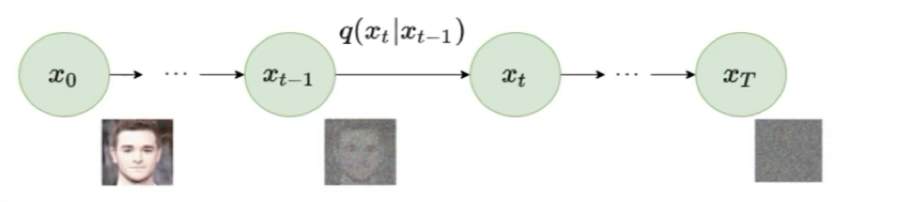
\includegraphics[width=\linewidth]{Fig1.png}
    \caption{Etapa de potencialização figurativa.}
    \label{fig1}
    \source{\textcite[p.~2]{ho2020denoising}.}
    \end{minipage}
\end{figure}

II – Etapa de realização figurativa: em movimento inverso, o modelo remove gradualmente o ruído anteriormente adicionado. Esse processo permite que os elementos visuais voltem a manifestar-se, não por simples recuperação dos elementos figurativos e plásticos da imagem inicial, mas por uma reconstrução orientada pelas regularidades estatísticas aprendidas durante o treinamento do modelo, da qual resulta uma combinação figurativa inédita. Observa-se, assim, um aumento progressivo da densidade sêmica, que torna possível o reconhecimento dos elementos visuais. Ao final desse percurso, obtém-se uma imagem que satisfaz critérios de coerência visual e de verossimilhança figurativa, dependentes, evidentemente, da densidade figurativa à qual o texto verbal (comando) remete (\Cref{fig2}).

\begin{figure}[h!]
    \centering
    \begin{minipage}{0.8\linewidth}
    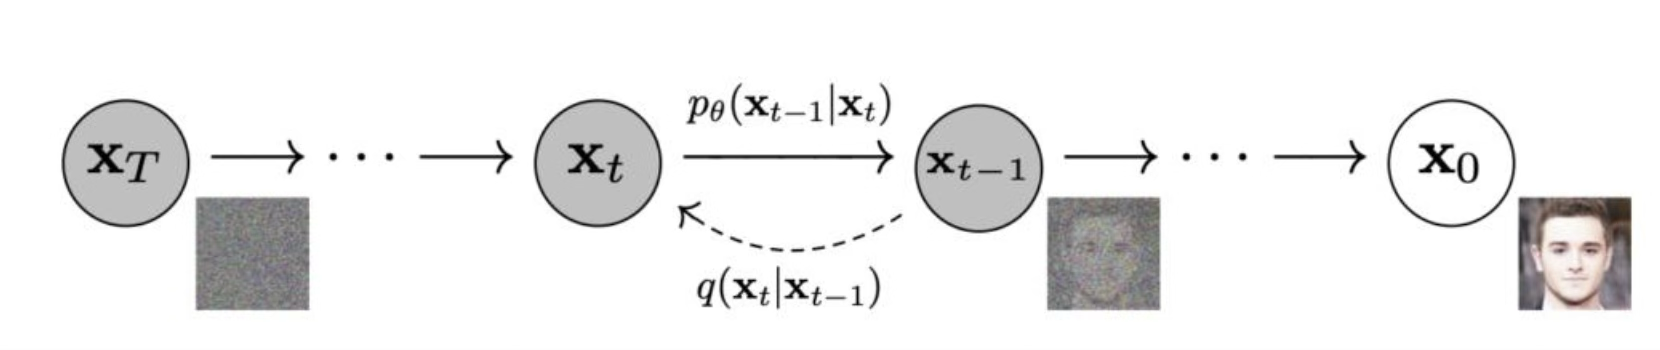
\includegraphics[width=\linewidth]{Fig2.png}
    \caption{ Etapa de realização figurativa.}
    \label{fig2}
    \source{\textcite[p.~2]{ho2020denoising}.}
    \end{minipage}
\end{figure}


É fundamental destacar que a segunda etapa — a de realização figurativa — mostra-se condicionada pelo comando verbal. O texto linguístico atua, assim, como um operador de modalização, restringindo e orientando as possibilidades figurativas disponíveis ao modelo. Na instância de geração do objeto semiótico, espera-se que o comando verbal instaure um dispositivo modal que configure um dever-ser e um dever-não-ser da figurativização, estabelecendo quais traços, formas, objetos e relações devem ou não ser realizados na manifestação da imagem produzida.

Por exemplo, diante do comando “crie uma imagem de um casal feliz caminhando na chuva no parque”, o modelo mobiliza o aprendizado estatístico adquirido na etapa 1 do processo de difusão (cf. \Cref{fig1}) para estabelecer associações entre os termos verbais e determinados traços figurativos.

Assim, o lexema “casal” remete à presença figurativa de dois corpos humanos, cuja diversidade corporal (constituição física, raça, idade) dependerá diretamente dos dados mobilizados no treinamento do modelo, pois o comando é aberto e não restringe as características visuais que devem ser associadas a corpo humano; “feliz” orienta a manifestação de elementos visuais que figurativizam expressões gestuais mais relaxadas e sorrisos; “caminhando” aciona organizações topológicas e eidéticas responsáveis pela construção do movimento corporal — posição de pernas e braços, postura geral e até o comportamento dos fios de cabelos —, as quais devem manter coerência com a ergonomia da ação; “chuva” remete a marcadores climáticos específicos; e, por fim, “parque” orienta a figurativização espacial do plano de fundo, mobilizando elementos como árvores, gramado, caminhos e, eventualmente, lagos.

Além do controle dos elementos figurativos, é possível fazer ainda alterações na plasticidade \cite{floch1979couleurs} do objeto visual a partir de comandos verbais. Em um teste exploratório realizado por nós no DALL·E, a partir dos comandos “imagem de um casal feliz caminhando na chuva no parque”, “imagem de um casal feliz caminhando na chuva no parque tirada por celular” e “imagem de um casal feliz caminhando na chuva no parque tirada por câmera analógica”, obtivemos os seguintes resultados, apresentados da esquerda para a direita na \Cref{fig3}.


\begin{figure}
    \centering
    \begin{minipage}{0.7\linewidth}
    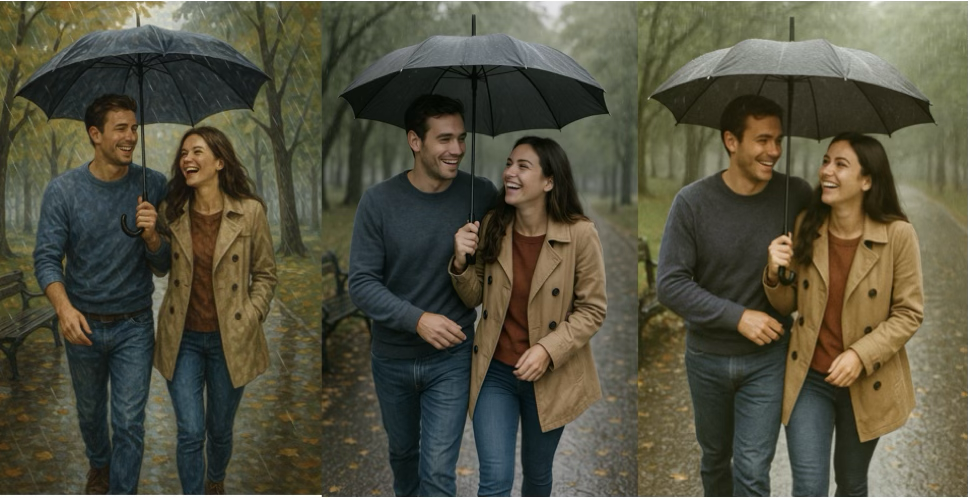
\includegraphics[width=\linewidth]{Fig3.png}
    \caption{Imagens de casal feliz caminhando no parque geradas pelo DALL·E.}
    \label{fig3}
    \source{DALL·E. Comandos <imagem de um casal feliz caminhando na chuva no parque> , <imagem de um casal feliz caminhando na chuva no parque tirada por celular> e <imagem de um casal feliz caminhando na chuva no parque tirada por câmera analógica>. 30 de ago. de 2025}
    \end{minipage}
\end{figure}

Quando o comando solicita uma “imagem tirada pelo celular”, nota-se que o modelo tende a acionar convenções associadas à fotografia digital, como maior nitidez, controle da iluminação, equilíbrio da saturação cromática e eliminação de elementos figurativos considerados visualmente incoerentes, a exemplo dos pingos de chuva que atravessavam o guarda-chuva. Nesse caso, a imagem gerada aproxima-se de uma correção técnica comum em fotografias de celular. Já quando o comando especifica que a imagem deve ser “tirada por câmera analógica”, o modelo passa a mobilizar elementos plásticos, marcadas por maior granulação, variações cromáticas menos estabilizadas, leves desfoques e efeitos de materialidade que remetem ao suporte fotoquímico. Esses traços plásticos alteram a textura da imagem e produzem efeitos de sentido associados à temporalidade, à memória e à autenticidade, próprios da fotografia analógica.

Dessa maneira, os comandos verbais não orientam apenas a figurativização dos elementos representados, mas modulam também questões próprias da enunciação que resultarão na maneira como a imagem se apresenta; no exemplo citado (\Cref{fig3}), como fotografia digital ou analógica. A escala, a proporção e a organização espacial dos elementos figurativos ajustam-se a essas orientações, evidenciando que o comando possivelmente atua simultaneamente na manifestação do plano da expressão e do plano do conteúdo.

No entanto, nem todas as escolhas realizadas pelas IA generativas de imagens dependem diretamente do comando verbal fornecido, pois muitas delas estão associadas à origem, composição e extensão do \textit{dataset} e aos algoritmos empregados no treinamento do modelo. É nesse contexto que emergem os estereótipos, derivados dos bancos de dados utilizados. Em nossos testes, por exemplo, ao inserir o comando com o sintagma nominal “um casal feliz”, o modelo figurativizou predominantemente um casal heterossexual, jovem e branco. Como observam \textcite{ho2020denoising}:

\begin{quote}
    os modelos generativos tendem a reproduzir os vieses presentes nos conjuntos de dados que os alimentam, sobretudo quando esses dados são coletados de forma automatizada na internet e carecem de rotulagem adequada. A ampla circulação de imagens produzidas por tais modelos contribui, inclusive, para a intensificação e a reprodução desses vieses ao longo do tempo \cite[p.~9]{ho2020denoising}.
\end{quote}

Os autores relacionam a questão da ampla circulação desses objetos visuais com o possível aumento dos vieses ao longo do tempo, uma vez que as IAGen não apenas alimentam seus bancos de dados com objetos semióticos produzidos por humanos, mas também com objetos produzidos por elas mesmas, em um ciclo infinito de reutilização de formas semióticas. Uma vez geradas, essas imagens podem voltar a fazer parte automaticamente do treinamento da máquina e, se não houver intervenção humana, continuarão a reforçar padrões discriminatórios, recrudescendo a presença de tais elementos do conteúdo e da expressão na geração de novos objetos semióticos visuais.

A questão do enviesamento decorre, assim, dos conjuntos de dados empregados no treinamento desses modelos que podem refletir desigualdades históricas de representação de corpos humanos. A recorrência de corpos brancos, jovens e heteronormativos como solução “padrão” para comandos semanticamente abertos evidencia que determinadas corporalidades ocupam uma posição privilegiada no espaço das virtualidades do sistema, enquanto outras permanecem sub-representadas ou associadas a contextos estereotipados. Assim, o que se apresenta como uma escolha automática do modelo corresponde às orientações ideológicas e axiológicas presentes na coleção de objetos semióticos constitutivos do \textit{dataset}.

Sob a perspectiva do enviesamento racial, tal fenômeno também aparece na orientação axiológica, regulando os critérios segundo os quais determinados corpos são tomados como formas semióticas prototípicas e associadas, na instância da manifestação textual, a certas tematizações de papéis sociais. Vale ressaltar, no entanto, que esse fenômeno não é restrito aos modelos de IA generativas, pois, ao analisar objetos semióticos visuais pertencentes ao banco de imagens da \textit{Shutterstock}, um repositório de imagens e fotografias hierarquizadas e organizadas por algoritmos, identificamos \cite{moraes2025semioticista} padrões de enviesamento racial semelhantes, em que somente corpos brancos eram associados ao papel temático da profissão de médico, estando os corpos negros confinados em uma espécie de “clandestinidade” do banco de imagens, cujo acesso só é possível a partir do uso da expressão linguística marcada “médico negro” no campo de buscas; essa valoração racista está presente nos diferentes modelos e usos de tecnologias, como demonstram as pesquisas de \textcite{carrera2021racismo,noble2022algoritmos} e \textcite{pasquale2015black}. Para uma melhor compreensão da questão nos modelos generativos, apresentaremos, a seguir, alguns testes realizados com o modelo DALL·E.

\section{Figuras e figuratividade nas imagens geradas pelo DALL·E}
Em consonância com as discussões anteriormente desenvolvidas acerca do enviesamento racial presente nos processos de figurativização gerados por IA generativas, a presente seção dedica-se ao exame do funcionamento do DALL·E, em sua quarta versão. Busca-se investigar, de modo mais detido, os mecanismos por meio dos quais o enviesamento racial se manifesta na geração de objetos semióticos visuais produzidos por esse modelo, a partir de testes que articulam a figurativização de corpos humanos a profissões socialmente investidas de maior ou menor valoração associada ao prestígio. O objetivo central consiste em analisar de que maneira corpos brancos e corpos negros são figurativizados nos objetos semióticos visuais por ele engendrados, observando as regularidades que emergem na distribuição dessas figuras.

Diante desse quadro, impõem-se algumas questões centrais: de que modo esses modelos figurativizam os corpos humanos no que concerne às questões raciais? Seriam os sucessivos treinamentos e a robustez de seus bancos de dados (\textit{big data}) suficientes para assegurar uma figurativização orientada por valores étnico-raciais? Ou, ao contrário, estariam tais sistemas reiterando estereótipos e padrões de discriminação estrutural e culturalmente enraizados na sociedade?


\subsection{Procedimentos metodológicos}

O nosso olhar circunscreve-se, neste momento, às questões raciais relacionadas especialmente às pessoas negras, objetivando compreender a interseção entre raça e status social. O desenho metodológico abrange testes com profissões consideradas valorizadas e não valorizadas. Os objetos semióticos visuais foram gerados por meio da plataforma DALL·E (versão 4), da OpenAI, em 10 de maio de 2025, utilizando a variante brasileira da língua portuguesa. Para cada uma das seis profissões selecionadas, foram elaborados dois comandos verbais (\textit{prompts}): um no gênero feminino e outro no masculino, totalizando doze (12) comandos (cf.\Cref{tab1}).

Os comandos foram deliberadamente formulados de modo minimalista, restringindo-se ao sintagma nominal (com ou sem especificador) que designa a profissão acompanhado do artigo indefinido correspondente (por exemplo, <uma médica> e <um médico>), com o propósito de reduzir a interferência de variáveis semânticas adicionais sobre os resultados, isolando, assim, o efeito da designação profissional na figurativização dos corpos.

A seleção das seis profissões analisadas — médico(a), professor(a) universitário(a), engenheiro(a) civil, faxineiro(a) de hospital, pedreiro(a) e catador(a) de lixo — baseou-se em um procedimento sistemático de coleta e análise de dados secundários, composto por três etapas: (i) levantamento inicial das profissões mais e menos valorizadas: realizou-se, em 5 de maio de 2025, uma busca no Google utilizando os seguintes sintagmas de pesquisa, em língua portuguesa (variante brasileira): "profissões mais prestigiadas no Brasil" e "profissões menos prestigiadas no Brasil". Foram considerados apenas os dez primeiros resultados orgânicos da primeira página do buscador, totalizando dez links analisados; (ii) estabelecimento dos critérios de inclusão e exclusão: foram selecionadas listas que explicitassem os critérios de classificação adotados (remuneração, reconhecimento social ou combinação desses fatores) e que fossem produzidas por, ou referenciadas em, instituições de pesquisa reconhecidas ou veículos nacionais de informação; (iii) sistematização e validação: a partir da compilação dos dados, identificaram-se as dez profissões mais recorrentes, cujos comandos foram testados no DALL·E.

Durante a fase de geração, verificou-se que o DALL·E não reconheceu adequadamente os comandos /um faxineiro/ e /uma faxineira/, possivelmente em razão da menor representatividade de dados em língua portuguesa. Para contornar essa idiossincrasia, o comando foi reformulado mediante a inclusão do especificador preposicionado de hospital, que restringe o referente, produzindo os resultados analisados. Os demais comandos não apresentaram problemas de reconhecimento semântico, ainda que, no caso de pedreira, o termo também possa remeter, em português, a um tipo de jazida mineral. O modelo, contudo, orientou-se de forma consistente pela acepção profissional.

Excluíram-se da lista as profissões cuja denominação coincidia com o termo ou a sigla em língua inglesa, como CEO, a fim de assegurar que a avaliação considerava exclusivamente o desempenho do modelo em língua portuguesa. Além disso, foram excluídas as profissões cujos comandos não foram reconhecidos pelo modelo, isto é, que não produziram imagens capazes de figurativizar de maneira reconhecível a ocupação solicitada.

Cabe salientar que a própria lista funciona como um indicador dos valores e das hierarquias compartilhados na semiosfera, uma vez que a distinção entre profissões socialmente valorizadas e não valorizadas não se restringe ao salário médio associado a cada ocupação, considerando também o prestígio social e a distinção historicamente construída entre trabalho intelectual e trabalho braçal, evidenciando os valores axiológicos atribuídos às diferentes profissões.

Com vistas a tornar o estudo analiticamente manejável, o \textit{corpus} foi deliberadamente reduzido a seis profissões: médico(a), professor(a) universitário(a) e engenheiro(a) civil, de um lado; faxineiro(a) de hospital, pedreiro(a) e catador(a) de lixo, de outro.

Tais procedimentos metodológicos resultaram na seguinte lista (\Cref{tab1}):

\begin{table}[htbp]
  \centering
  \caption{Comandos verbais (prompts) utilizados para a geração de imagens no DALL·E.}
  \label{tab1}
  \begin{tabular}{lll}
    \toprule
    \small
    Profissão & Comando (feminino) & Comando (masculino) \\
    \midrule
    Médico(a) & <uma médica> & <um médico> \\
    Professor(a) universitário(a) & <uma professora universitária> & <um professor universitário> \\
    Engenheiro(a) civil & <uma engenheira civil> & <um engenheiro civil> \\
    Faxineiro(a) de hospital & <uma faxineira de hospital> & <um faxineiro de hospital> \\
    Pedreiro(a) & <uma pedreira> & <um pedreiro> \\
    Catador(a) de lixo & <uma catadora de lixo> & <um catador de lixo> \\
    \bottomrule
  \end{tabular}
  \source{Elaboração própria.}
\end{table}

Todos os comandos foram testados duas vezes, gerando, assim, vinte e quatro (24) resultados. Como não houve diferenças significativas entre ambos os testes no que diz respeito à figurativização racial, optou-se por usar os resultados do primeiro teste, restringindo-se, portanto, a doze (12) objetos semióticos visuais.

Salienta-se que os resultados aqui apresentados não pretendem generalizar o funcionamento de todos os modelos de IA generativa, nem mesmo de todas as versões do DALL·E, uma vez que cada sistema opera com algoritmos, conjuntos de dados e procedimentos de curadoria específicos. Reconhece-se, por fim, que a análise aqui desenvolvida tem caráter exploratório e se insere em um programa de pesquisa mais amplo sobre a atuação de agentes maquínicos na geração da significação nos objetos semióticos, práticas e formas de vida \cite{moraes2021nocao,moraes2024semiotica,moraes2025semioticista,moraesdesousa2026construction,moraesdesousa2026generative}.

Passamos, agora, à apresentação dos resultados gerados pela inteligência artificial e de suas análises.


\subsection{Análise do viés racial em imagens geradas pela inteligência artificial}

A seguir, reproduzimos os objetos semióticos visuais gerados durante o teste com o DALL·E (\Cref{fig4,fig5,fig6,fig7,fig8,fig9}).

\begin{figure}[htbp]
    \centering
    \begin{minipage}[t]{0.48\linewidth}
        \centering
        \vfill
        
\includegraphics[width=\linewidth]{Fig4.png}
        \caption{Médica e médico gerados pelo DALL·E.}
        \label{fig4}
        \source{DALL·E. Comandos <uma médica> e <um médico>. 10 de maio de 2025.}
    \end{minipage}
    \hfill
    \begin{minipage}[t]{0.48\linewidth}
        \centering
        \vfill
        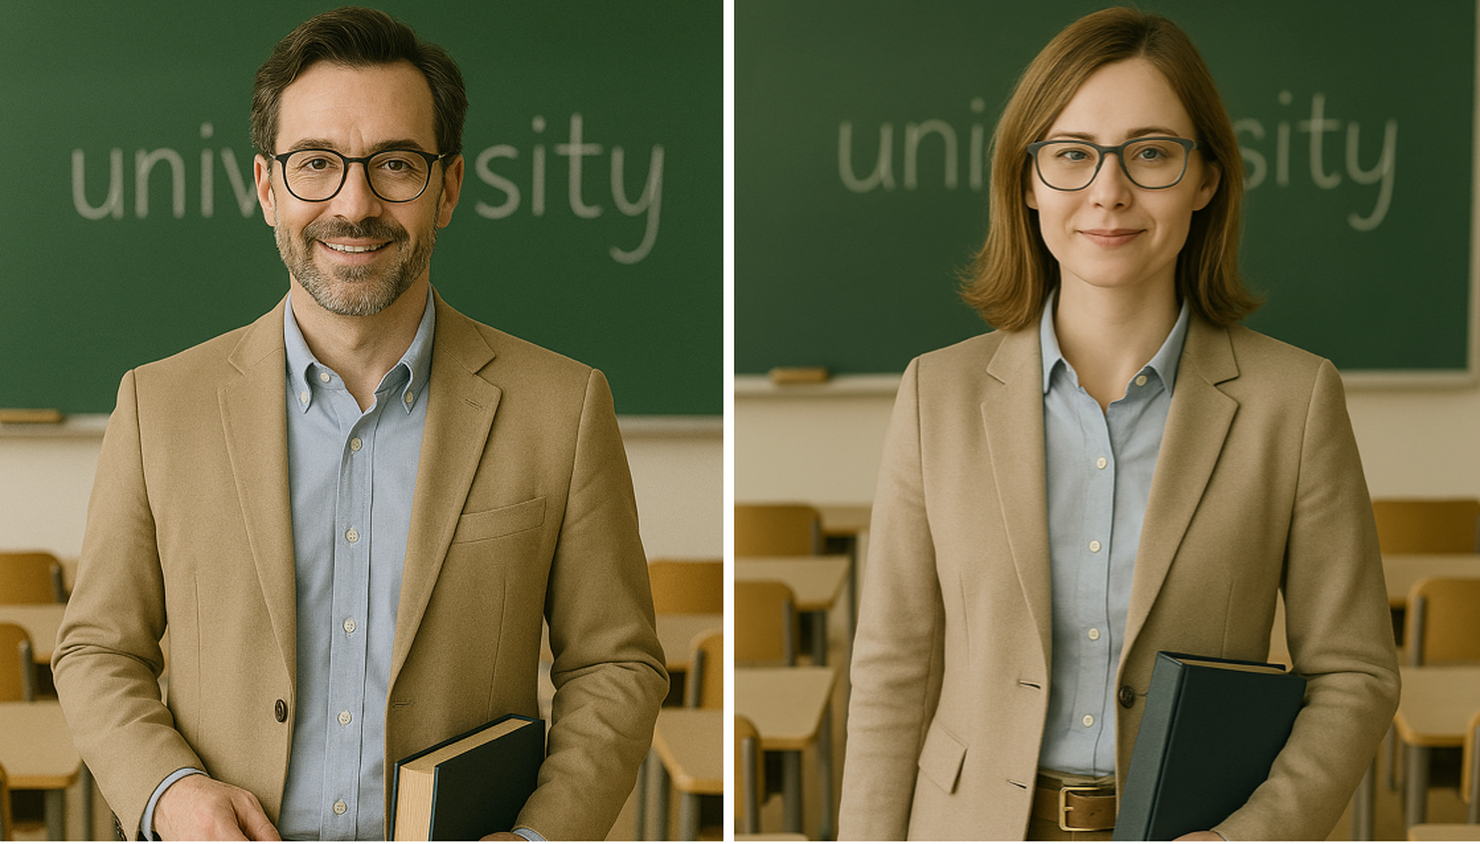
\includegraphics[width=\linewidth]{Fig5.png}
        \caption{Professor universitário e professora universitária gerados pelo DALL·E.}
        \label{fig5}
        \source{DALL·E. Comandos <um professor universitário> e <uma professora universitária>. 10 de maio de 2025.}
    \end{minipage}
\end{figure}

\begin{figure}[htbp]
    \centering
    \begin{minipage}[t]{0.48\linewidth}
        \centering
        \vfill
        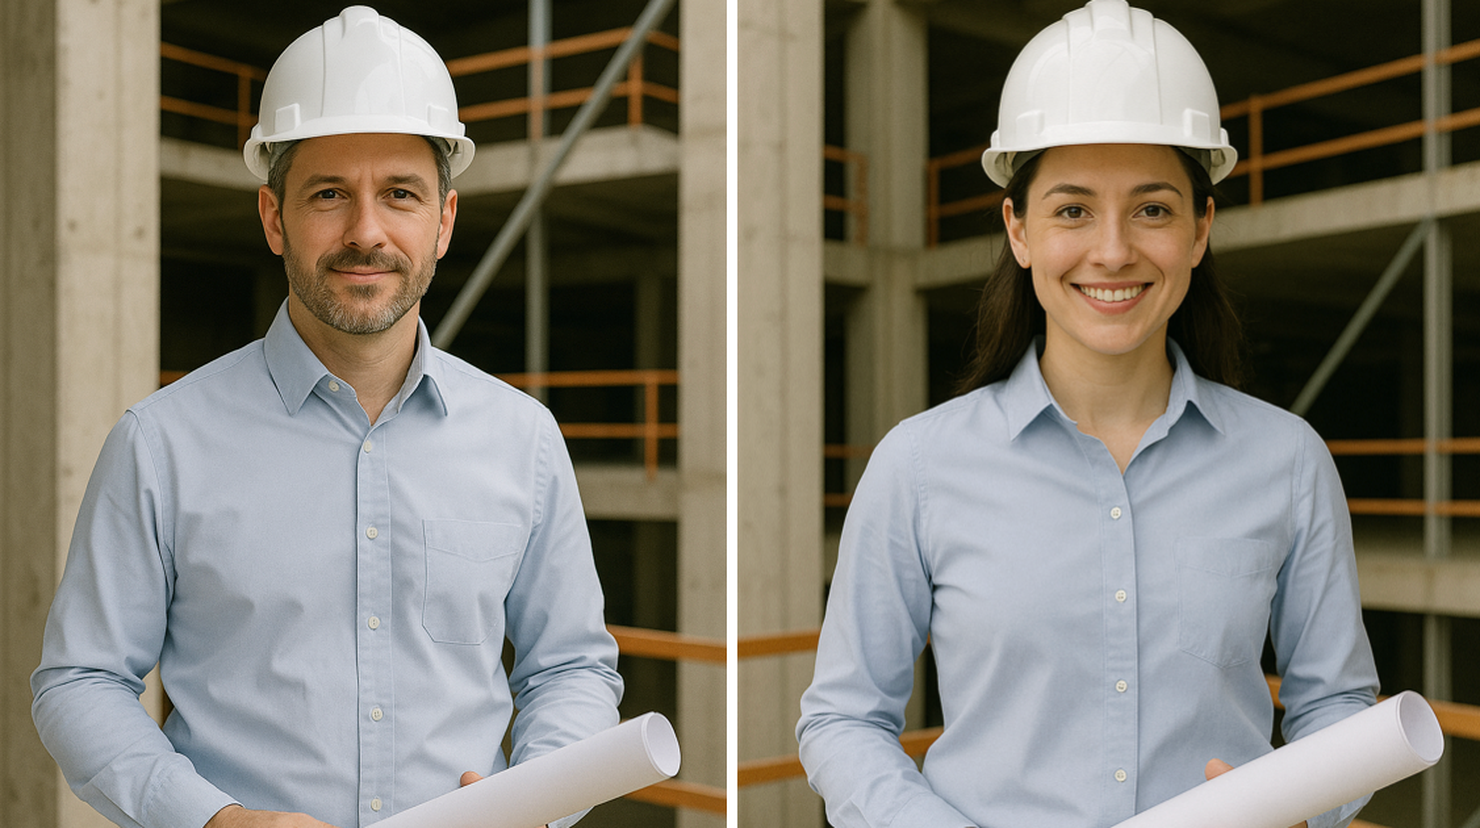
\includegraphics[width=\linewidth]{Fig6.png}
        \caption{Engenheiro civil e engenheira civil gerados pelo DALL·E.}
        \label{fig6}
        \source{DALL·E. Comandos <um engenheiro civil> e <uma engenheira civil>. 10 de maio de 2025.}
    \end{minipage}
    \hfill
    \begin{minipage}[t]{0.48\linewidth}
        \centering
        \vfill
        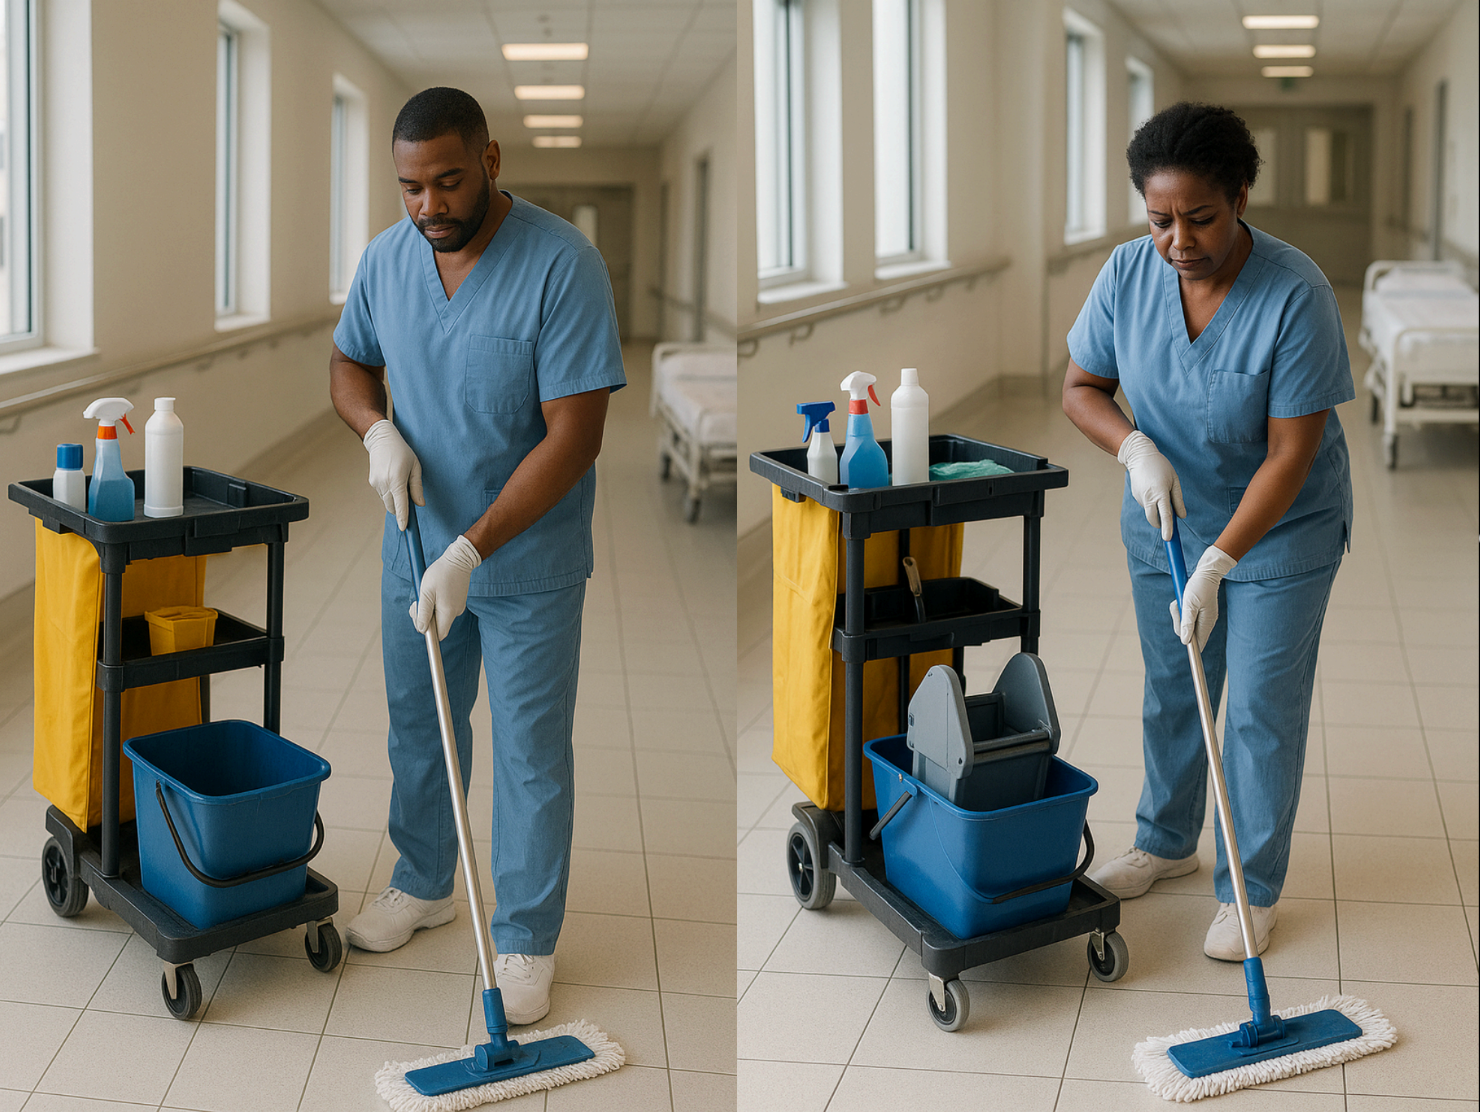
\includegraphics[width=\linewidth]{Fig7.png}
        \caption{Faxineiro e faxineira de hospital gerados pelo DALL·E.}
        \label{fig7}
        \source{DALL·E. Comandos <um faxineiro de hospital> e <uma faxineira de hospital>. 10 de maio de 2025.}
    \end{minipage}
\end{figure}

\begin{figure}[h!]
    \centering
    \begin{minipage}[t]{0.48\linewidth}
        \centering
        \vfill
        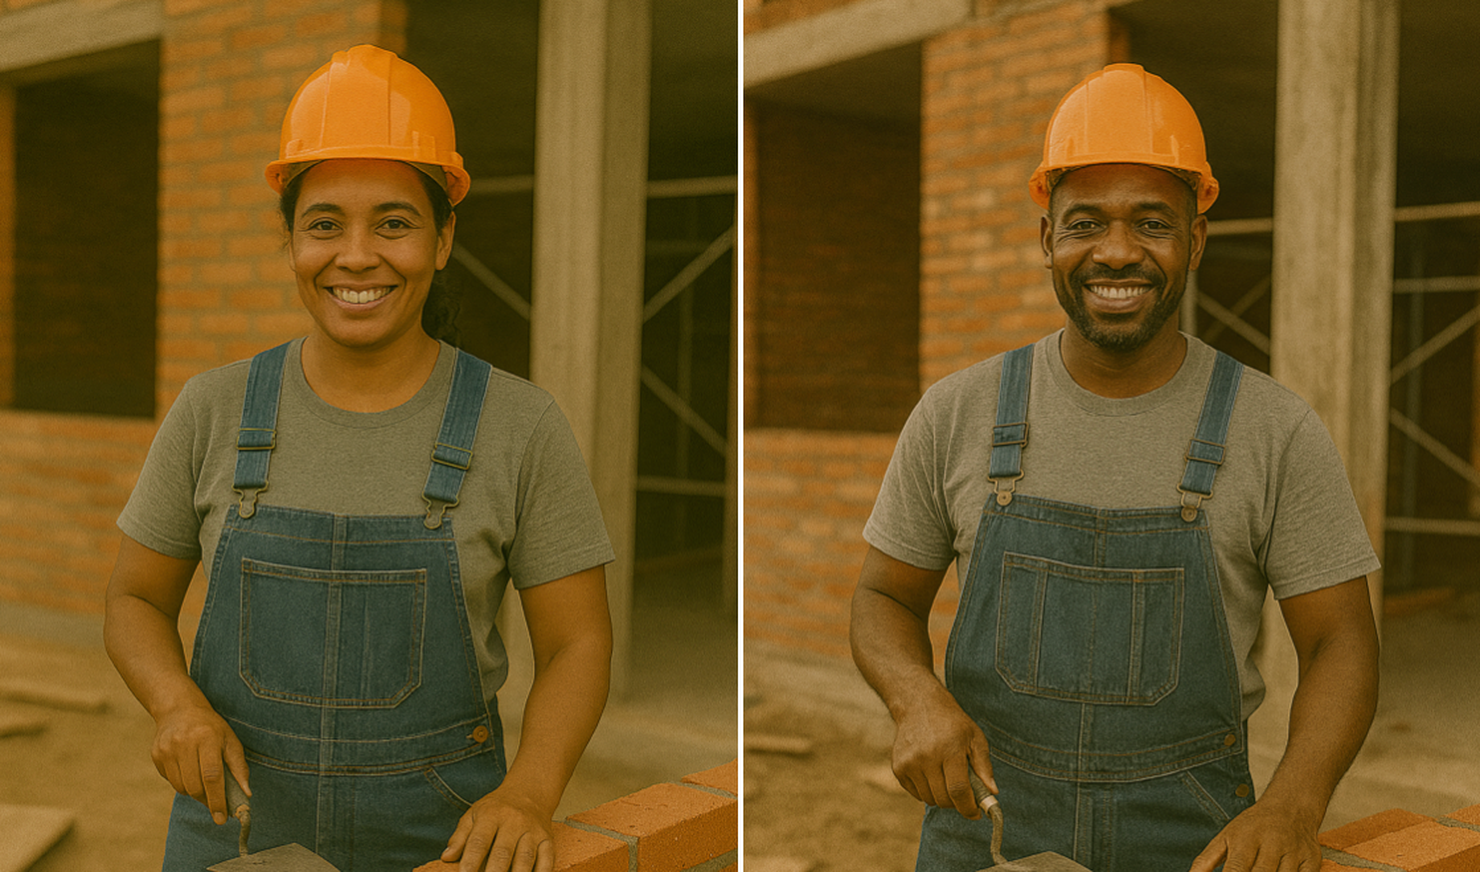
\includegraphics[width=\linewidth]{Fig8.png}
        \caption{Pedreira e pedreiro gerados pelo DALL·E.}
        \label{fig8}
        \source{DALL·E. Comandos <uma pedreira> e <um pedreiro>. 10 de maio de 2025.}
    \end{minipage}
    \hfill
    \begin{minipage}[t]{0.48\linewidth}
        \centering
        \vfill
        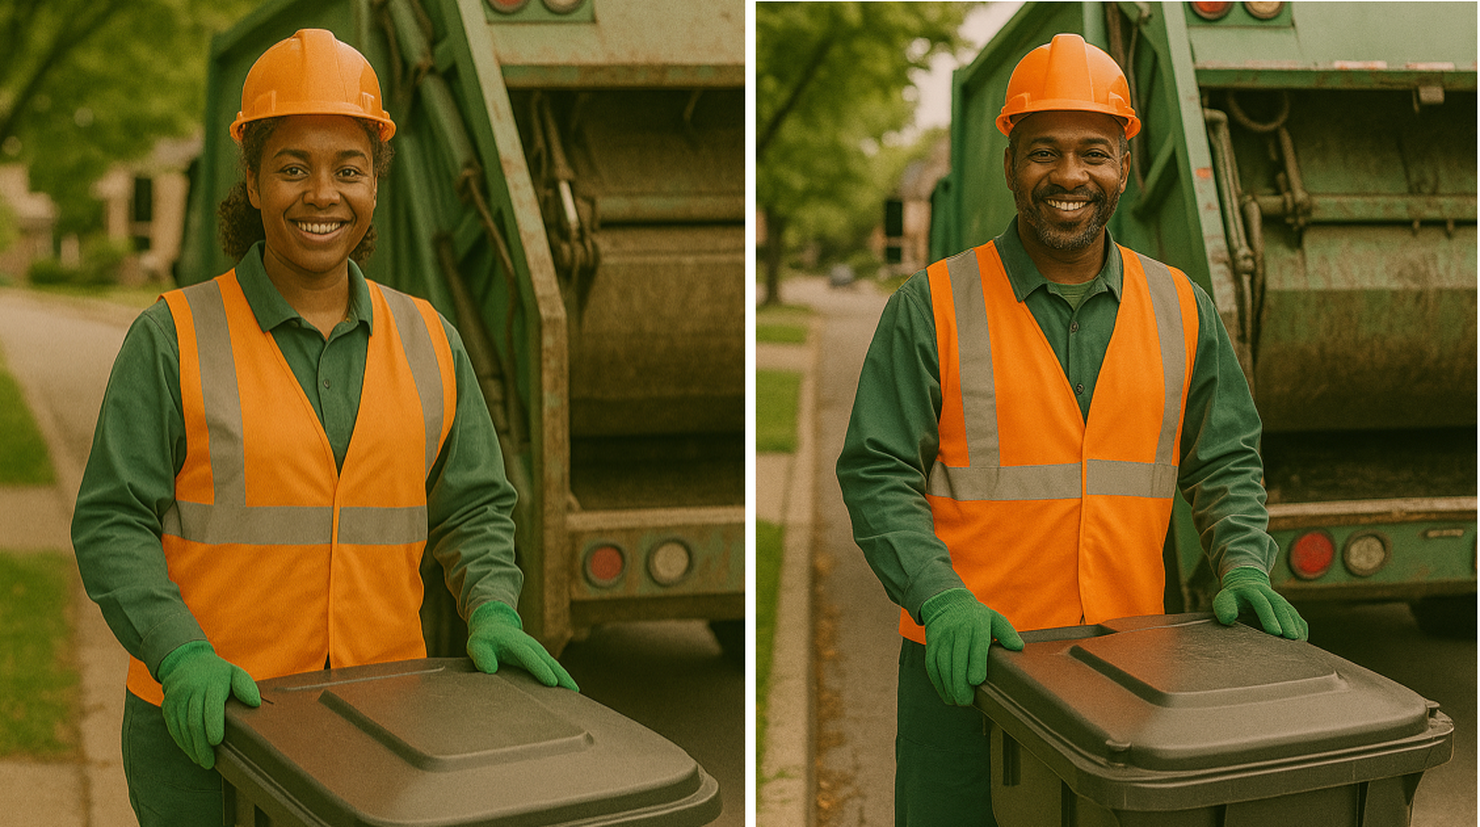
\includegraphics[width=\linewidth]{Fig9.png}
        \caption{Catadora de lixo e catador de lixo gerados pelo DALL·E.}
        \label{fig9}
        \source{DALL·E. Comandos <uma catadora de lixo> e <um catador de lixo>. 10 de maio de 2025.}
    \end{minipage}
\end{figure}

A análise dos resultados mostra que, em todos os objetos semióticos gerados, a IA figurativizou elementos visuais associados à profissão indicada no comando verbal escrito; por exemplo, se o comando foi "médico", o resultado apresentou corpos humanos vestidos com roupas brancas e estetoscópio sobre os ombros (\Cref{fig4}). Para outras, a figurativização da profissão aparece também no plano de fundo, contribuindo para a construção do cenário: os professores universitários são representados em uma sala com quadro ao fundo e objetos que remetem a cadeiras escolares (\Cref{fig5}).

De modo geral, observa-se que, em aproximadamente metade dos objetos semióticos analisados (\Cref{fig4,fig7,fig9}), os corpos humanos são figurativizados por meio de uniformes profissionais padronizados, tomados como representativos das respectivas profissões. Cabe, entretanto, uma ressalva: em quase todas essas imagens, inscrevem-se marcas de um enunciador não brasileiro, apesar de os comandos terem sido formulados em língua portuguesa do Brasil. Isso pode ser observado na palavra "university" presente atrás dos professores universitários (\Cref{fig5}), além da construção visual do espaço das diferentes imagens. Tal descompasso torna-se particularmente evidente no caso dos catadores de lixo (\Cref{fig9}), cuja indumentária — composta por luvas verdes, macacão verde com detalhes em laranja e cinza, além de capacete laranja — não corresponde aos usos e às práticas correntes no contexto brasileiro.

Nas demais imagens, os corpos humanos são figurativizados por meio de vestimentas comuns, não explicitamente associadas a um uniforme profissional. Observa-se, contudo, uma recorrência significativa: nos casos dos médicos (\Cref{fig4}), engenheiros civis (\Cref{fig6}) e professores universitários (\Cref{fig5}), todos os sujeitos são representados com camisas sociais azuis, o que sugere a construção temática de sobriedade e formalidade para profissões de maior prestígio. Ademais, apenas os professores universitários aparecem usando óculos (\Cref{fig5}), acessório que, no plano figurativo, funciona como marcador de intelectualidade, reforçando estereótipos visuais historicamente vinculados à atividade acadêmica.

As profissões socialmente consideradas valorizadas foram figurativizadas, sem nenhuma exceção, por corpos brancos, ao passo que as profissões associadas a menor prestígio social foram figurativizadas por corpos negros de maneira sistemática. Tal regularidade evidencia uma correlação estável entre raça e hierarquização profissional no interior dos objetos semióticos visuais produzidos pelo modelo. Na imagem que representa os catadores de lixo (\Cref{fig9}), por exemplo, os corpos são construídos a partir de traços semânticos visuais que constroem a figura do corpo negro e a temática da negritude, por meio da recorrente combinação dos elementos visuais /pele escura/ + /cabelo crespo/ + /lábios carnudos/ + /nariz largo/.

Esses traços, ao serem associados a funções socialmente desvalorizadas — e, de modo correlato, ao se ausentarem das figurativizações vinculadas às profissões de maior prestígio — constituem uma isotopia visual do racismo, na qual a hierarquização racial se estabiliza e se naturaliza simultaneamente nos planos da expressão e do conteúdo.

Tais resultados convergem com as análises do sociólogo brasileiro \textcite{souza2017elite}, especialmente em sua obra A elite do atraso: da escravidão à Lava Jato, nas quais o autor argumenta que a estrutura social brasileira, marcada pela herança escravocrata, tende a concentrar as elites, espaço social ocupado majoritariamente por pessoas brancas, em profissões de caráter intelectual, administrativo e socialmente reconhecidas como qualificadas, enquanto a população negra permanece desproporcionalmente associada a trabalhos corporais, precarizados e repetitivos. Essa configuração histórica encontra respaldo também nas análises da historiadora \textcite{schwarcz1993espetaculo}, que, em \textit{O espetáculo das raças: cientistas, instituições e questão racial no Brasil} (1870–1930), demonstra como discursos científicos e institucionais contribuíram para consolidar hierarquias que associavam corpos negros à inferioridade social e a posições subalternizadas na divisão do trabalho. Sob tal perspectiva, pode-se afirmar que esses sujeitos são frequentemente privados das condições necessárias para adquirir a competência modal do poder-fazer indispensável à realização do programa narrativo da ascensão social.

Nos resultados do DALL·E., todas as pessoas brancas são figurativizadas com cabelos longos, lisos e cuidadosamente alinhados (\Cref{fig4,fig5,fig6}). No caso das mulheres, apenas a médica (\Cref{fig4}) aparece com o cabelo preso; ainda assim, trata-se de um penteado que permite uma maior visualização dos fios. Já a engenheira (\Cref{fig6}) e a professora universitária (\Cref{fig5}) são representadas com os cabelos soltos, elementos que podem ser associados, no contexto de nossa sociedade, à feminilidade e à elegância.

Em contraste com essas figurativizações, as mulheres negras, quando representadas com cabelos longos — como a pedreira (\Cref{fig8}) e a catadora de lixo (\Cref{fig9}) — aparecem sistematicamente com os fios presos. Não se observa, por exemplo, a realização de um cabelo black power volumoso, forma historicamente associada à afirmação estética e política da negritude. A faxineira do hospital (\Cref{fig7}), única exceção quanto ao uso de cabelos soltos, é figurativizada com os fios muito curtos, o que reforça a contenção da figura capilar visual da estética negra. Vale ressaltar que o mesmo acontece com os corpos masculinos: os homens negros (\Cref{fig7,fig8,fig9}) foram figurativizados com cabelos raspados, enquanto os homens brancos (\Cref{fig4,fig5,fig6}) com fios mais longos.

Essa recorrência de formas não é fortuita. No interior dos sistemas axiológicos que estruturam a cultura ocidental, o corpo negro tem sido historicamente construído como um signo disfórico, portador de valores negativos, ao passo que o corpo branco se afirma euforicamente como o "nós", isto é, como medida implícita do padrão normativo, prototípico e desejável. É nessa mesma direção que nossas reflexões encontram ressonância nas análises da psicanalista Isildinha \textcite{nogueira1998significacoes}, que, em sua tese de doutorado intitulada \textit{Significações do corpo negro}, procura evidenciar como a corporalidade negra é investida de sentidos socialmente não aceitos. Como afirma a autora:

\begin{quote}
     O negro, no entanto, é aquele que traz a marca do 'corpo negro', que expressa, escatologicamente, o repertório do execrável que a cultura afasta, pela negativação. Vítima das representações sociais que investem sua aparência daqueles sentidos que são socialmente recusados, o negro se vê condenado a carregar na própria aparência a marca da inferioridade social \cite[p.~44]{nogueira1998significacoes}.
\end{quote}

O controle desses elementos figurativos não decorre da descrição verbal fornecida pelos comandos verbais simples e genéricos (por exemplo: <uma faxineira de hospital> ou <um faxineiro de hospital>), mas antes de uma seleção hierárquica operada pelos agentes maquínicos, isto é, pelos algoritmos e pelos conjuntos de dados que estruturam o modelo. Por meio de operações estatísticas, tais agentes organizam e hierarquizam, no plano da expressão, combinações recorrentes de figuras e traços visuais, fazendo convergir profissões socialmente desvalorizadas com corpos negros e com marcas plásticas específicas — como cabelos raspados, curtos ou rigidamente presos —, ao passo que, nos contextos de maior prestígio, essas mesmas marcas são ausentes.

Há, ainda, uma outra dimensão relevante a ser observada, relativa à aspectualidade manifestada nas imagens produzidas. Nas profissões socialmente menos valorizadas, os corpos negros são figurativizados em plena atividade, em um fazer: os faxineiros (\Cref{fig7}) aparecem posicionando o rodo como se estivessem limpando o chão, flagrados no curso da ação; os pedreiros (\Cref{fig8}) são representados no ato de construir uma parede; e os catadores de lixo (\Cref{fig9}) estão manipulando diretamente a caçamba na rua. Trata-se, portanto, de uma aspectualidade de natureza processual e modalizada pelo fazer.

Em contraste, nas profissões associadas a maior prestígio social, observa-se um distanciamento da modalidade do fazer. Os professores universitários (\Cref{fig5}), embora situados em uma sala de aula, encontram-se em um espaço desocupado: seguram um livro, enquanto ao fundo se lê a palavra "university", mas não escrevem no quadro nem interagem com alunos. De modo semelhante, os engenheiros civis (\Cref{fig6}) são posicionados fora do canteiro de obras vazio e portam um papel que remete a um projeto, sem qualquer envolvimento direto com a execução material da construção. O caso dos médicos (\Cref{fig4}) é ainda mais emblemático: o espaço ao fundo é indeterminado, os braços estão cruzados e nenhum instrumento de trabalho é efetivamente mobilizado — o estetoscópio, repousando sobre os ombros, funciona antes como figura que remete ao conteúdo identitário do que como ferramenta de uma prática em curso.

Enquanto os corpos negros associados às profissões socialmente desvalorizadas são figurativizados sob a égide do fazer, aqueles vinculados às ocupações de maior prestígio são modalizados pelo ser. Nesses casos, o corpo branco basta-se a si mesmo como elemento visual da expressão que desencadeia no plano do conteúdo o significado, por exemplo, de médico: o jaleco e o estetoscópio sobre seu corpo funcionam como figuras autossuficientes e essenciais para a constituição do seu papel temático, dispensando, assim, a figurativização do sujeito em uma prática em curso que correspondesse à profissão.

Tal distinção encontra respaldo na história da iconografia ocidental. A título de exemplificação, podemos recuperar as representações das divindades, como Asclépio, deus da cura e da medicina, cujo tema da autoridade é construído pela figurativização de sua própria presença e os valores que lhe são associados. Em contraste, nos objetos visuais que remetem ao período da escravidão no Brasil, os corpos negros aparecem quase invariavelmente figurativizados no trabalho forçado. Esses exemplos contribuem para nosso argumento a respeito da estreita relação entretida entre dados (\textit{dataset} e \textit{big data}) e sociedade \cite{moraes2021nocao,moraes2024semiotica}; enquanto objetos semióticos, portadores de valores, tais artefatos, por serem estatisticamente manipulados, constroem e reforçam as isotopias e temas presentes no centro da semiosfera em que foram produzidos, desconsiderando outras significações geradas em suas periferias.

A presente discussão remete-nos ao conceito de semiosfera, tal como compreendido pelo semioticista \textcite{lotman2019semiosfera}. Para o autor, a semiosfera corresponderia à cultura semiotizada, uma espécie de “espaço-tempo” semiótico vivo, estruturado dinamicamente a partir da interação entre um centro e uma periferia, que são simultaneamente separados e unidos por fronteiras. O centro dessa semiosfera é regido pela presença de uma linguagem ou norma dominante, na qual se concentram os valores mais conservadores que definem as práticas e as formas de vida consideradas aceitáveis na sociedade. Dessa maneira, para avançarmos no desenvolvimento de IAs mais éticas e plurais na próxima década, será preciso considerar as periferias da semiosfera na construção de coleções de dados destinadas ao treinamento desses modelos.


\section{Epílogo}

Contrariando o arquétipo da inteligência artificial neutra, objetiva e universal, a análise desenvolvida neste artigo aponta para um problema de ordem epistemológica: modelos de IA generativa funcionam a partir de quadros axiológicos específicos e hegemônicos próprios do centro da semiosfera, presentes em seus \textit{datasets}. Os dados empregados no treinamento do DALL·E — bem como os critérios algorítmicos que organizam sua combinatória — portam conteúdos que manifestam hierarquias historicamente cristalizadas, oriundas de epistemologias eurocentradas, coloniais e racializadas, que estão presentes no próprio sistema de significação, uma vez que tais dados não são construídos \textit{ex nihilo}.

Ao figurativizar corpos brancos como elementos figurativos pertencentes às profissões socialmente valorizadas e corpos negros como operadores do fazer nas ocupações desprovidas de prestígio, os modelos de IA estabilizam tais formas nesses usos e conferem-lhes o estatuto de norma semiótica. Dessa maneira, o “vir a ser” dessas tecnologias se assenta no valor de continuidade, ao evidenciar que os modelos de geração de imagens lançam mão de correlações entre expressão e conteúdo já estabilizadas por práticas realizadas pelas classes dominantes no interior da semiosfera, reproduzindo axiologias responsáveis pela construção de estereótipos que são anteriores à sua própria existência.

Vale lembrar que esses objetos semióticos visuais produzidos por IAGen, como mostramos no presente artigo, ou aqueles constituintes dos bancos de imagens, como no exemplo citado de \textcite{moraes2025semioticista}, ajudam a construir o imaginário sociocultural e a memória coletiva compartilhados pelos sujeitos inseridos em uma dada semiosfera e fortalecem a discriminação de determinados grupos minorizados, excluindo-os de certas esferas sociais, pois tais objetos semióticos visuais circulam em campanhas publicitárias, materiais didáticos, mídias sociais, notícias e assim por diante.

O estudo de tecnologias, como os modelos de inteligência artificial generativa, requer dos(as) analistas das humanidades um posicionamento crítico, que reconheça as implicações de seus usos e os valores produzidos ou reiterados, bem como a estreita aproximação entre dados, capitalismo e significação dentro de um ecossistema tecnossemiótico, em que os agentes maquínicos, as instituições privadas e o \textit{big data} atuam em colaboração na geração da significação emergentes das cenas práticas e da estruturação das formas de vida.

É nesse horizonte que se impõe como desafio a construção de uma semiótica da inteligência artificial, como tarefa teórica e política para semioticistas, analistas do discurso e humanistas digitais, que seja capaz de, por um lado, discutir as significações que esses sistemas reproduzem e fazem durar — ou melhor, perdurar — na semiosfera, bem como contribuir para o desenvolvimento de modelos a partir de uma perspectiva epistemológica do Sul Global\footnote{O Sul Global não designa exatamente uma localização geográfica, mas antes um posicionamento epistemológico contra-hegemônico, que propõe uma crítica radical à hegemonia predominante de determinadas culturas na ciência, na cultura, na tecnologia, entre outros domínios.}.

\printbibliography\label{sec-bib}
% if the text is not in Portuguese, it might be necessary to use the code below instead to print the correct ABNT abbreviations [s.n.], [s.l.]
%\begin{portuguese}
%\printbibliography[title={Bibliography}]
%\end{portuguese}


\begin{dataavailability}
\txtdataavailability{databody} % options: dataavailable, dataonly, databody, datanotav, nodata
\end{dataavailability}


\end{document}

